\biohead{Kathleen Munday}{Kathleen_Munday}{ }
%\section{Kathleen Munday}\label{Kathleen_Munday}
%\begin{center}
%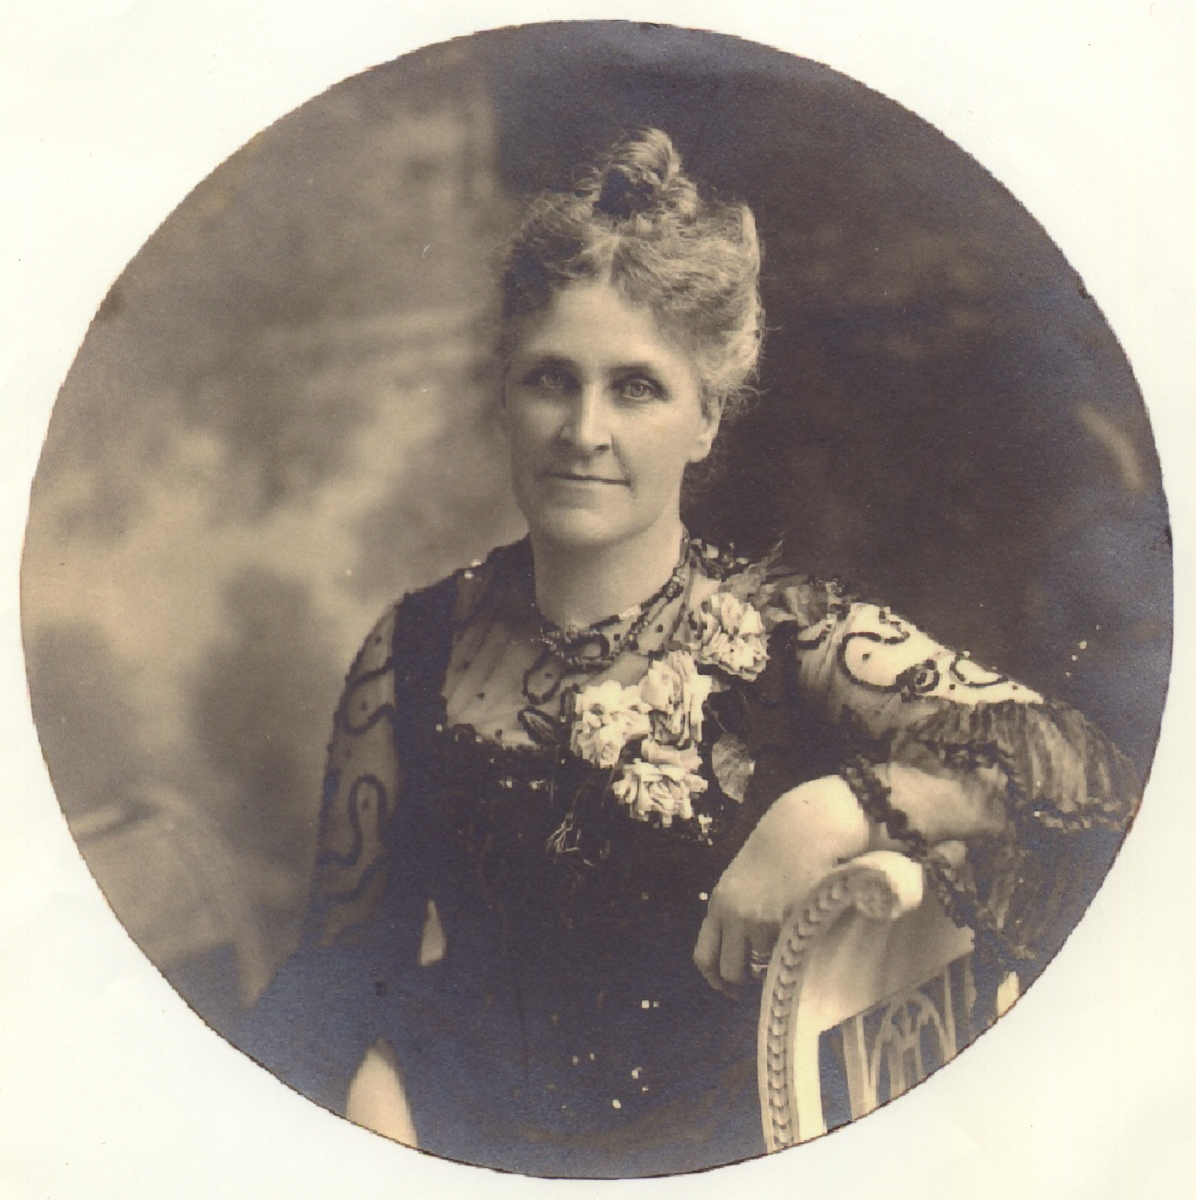
\includegraphics[width=0.8\linewidth]{photos/Kathleen_Munday}
%\end{center}

Katheen Munday  was born at 8 Shalston Villas, Surbiton (at 3.30pm, on 5th November 1882 - 17 September 1963) [ Munday family tree.  ↑ General Register Office, Birth Certificate BXCF517663. ↑ 3.0 3.1 John Hill Munday Family bible] and christened on 18 July 1883 in Surbiton.  She was the second daughter of John Hill Munday, who was a partner in a firm of solicitors in London. Her siblings were Nora Katie Munday (1881 - 1972), Mildred Mary Munday (1884 - 1974), Ralph Munday (1885-1962) and Margery Munday (1887 - ?). They lived at The Mendips, Surbiton, Surrey.  She was educated at Cheltenham Ladies College, but like most middle class women of her generation did not receive a higher education, nor did she seek employment after finishing school. She was a very accomplished wood carver and artist and received a medal for her fine work (see photographs). She met James Denton Barker when she was on holiday at Ilkley and they married just before the outbreak of the first World War on 4th April 1914 at the Wandsworth Registry Office. The notice in the Times read:
[↑ From The Times:]
"The Marriage of Miss Kathleen Munday, second daughter of Mr. and Mrs. J.H.Munday, of Cedar Lodge, St.Johns Road, Putney, with Mr. James Denton Barker, of Liverpool, took place very quietly in London on the 4th inst. The bride was married in her travelling dress of blue serge, with a black tagal hat trimmed with a pale blue ostrich feather and a pink rose. Mr and Mrs J. Denton Barker left immediately after the ceremony for the Yorkshire moors and the Lake District, where the honeymoon is being spent, prior to taking up their residence in Liverpool. A reception was held on the previous day by the bride's mother, which was attended by a number of guests, when the many very handsome presents were on view."
 Early the following year their first son, Mead, was born, followed a year and a half later by Ralph (p.\pageref{Ralph_Munday_Denton-Barker}), and then Virginia (p.\pageref{Virginia_Kathleen_Denton_Barker}) in 1919.
For most of their married life, James and Cathleen lived in Birkenhead (Beechwood, Mt. Pleasant) and in later years in Harpenden, Hertfordshire. She then moved to Leeds to live near her family and died on 17 September 1963. [death ref] [probate ref/quote  Probate: Barker Kathleen of Laurel Bank, Templar lane, Stanks, Leeds widow died 17 September 1963 at The Grand Infirmary, Leeds. Probate Wakefield 14 November to Virginia Kathleen Denton Grebenik (wife of Eugene Grebenik) and D. McCandlish Bell solicitor. (pounds)29,594.8s.]
